     %\ \
     %\begin{minipage}[b]{0.49\textwidth}
     %  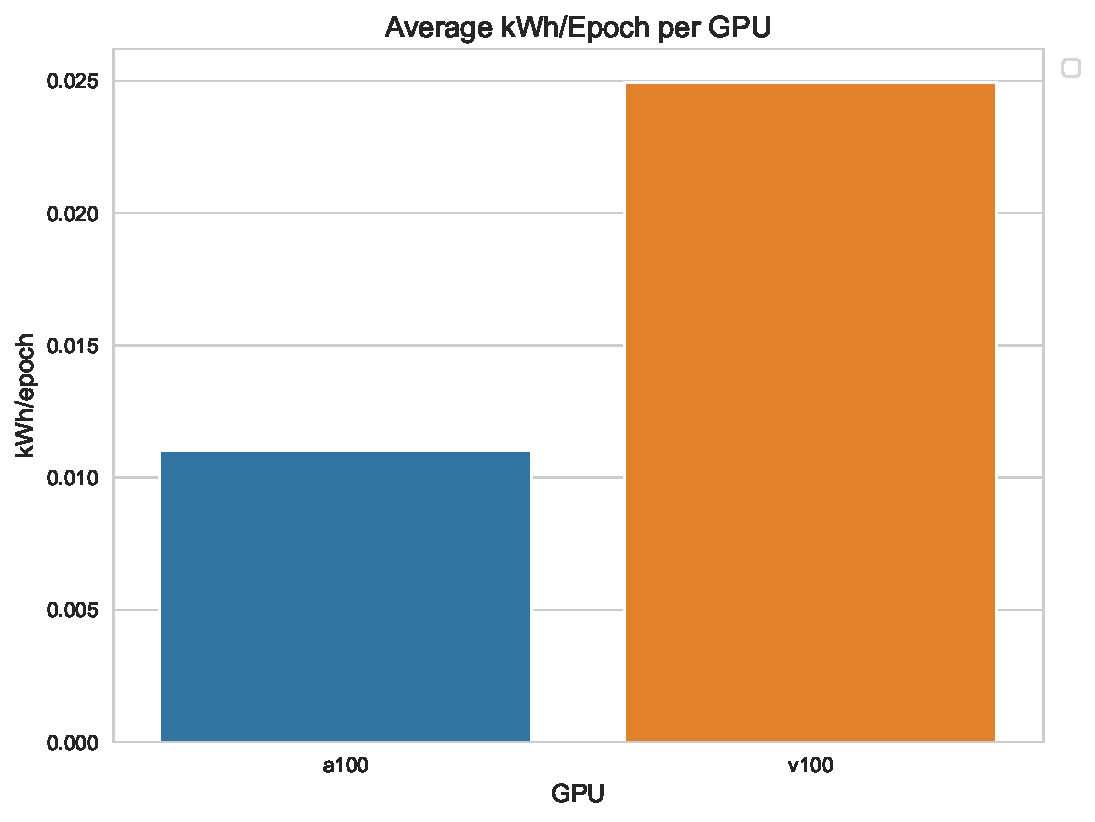
\includegraphics[width=1.0\linewidth]{images/average_kWh_per_epoch.pdf}
     %   {\bf (B)} average kWh per epoch
     %\end{minipage}

     %\begin{minipage}[b]{0.49\textwidth}
     %  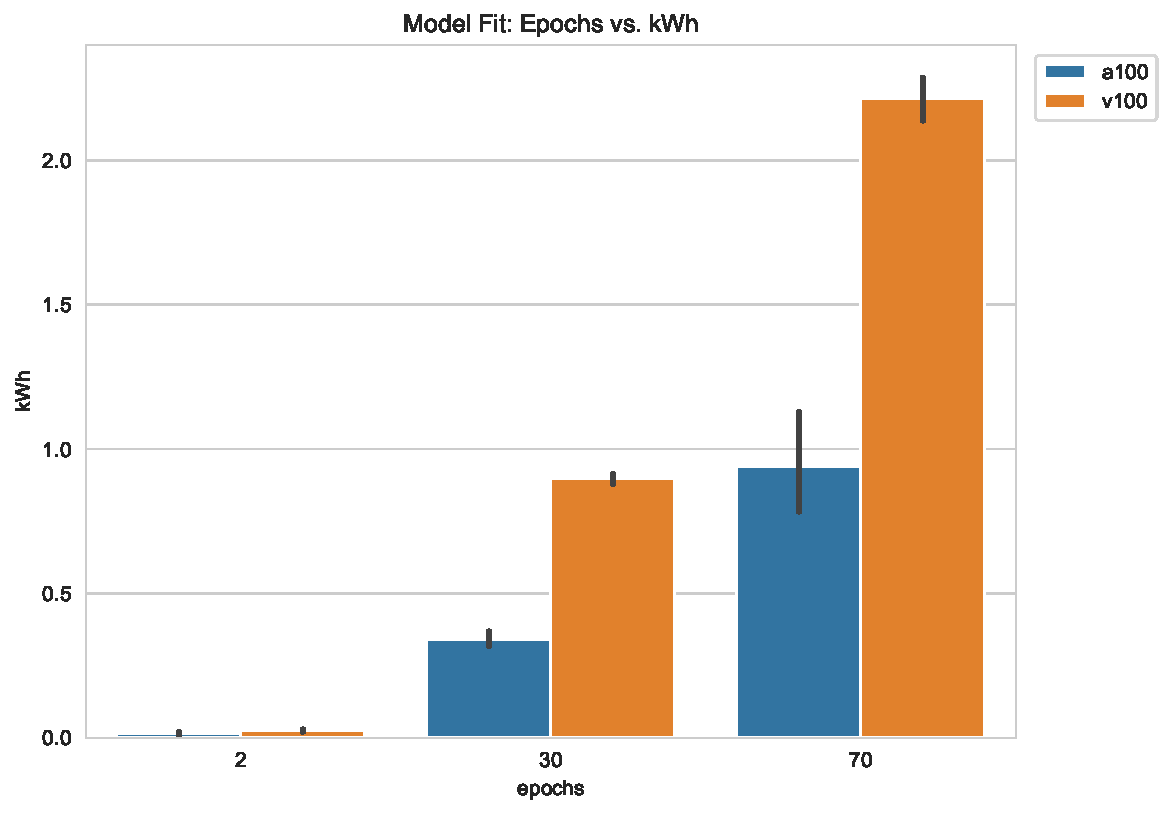
\includegraphics[width=1.0\linewidth]{images/model_fit_epoch_vs_watts.pdf}
     %   {\bf (C)} model fit epoch vs watts
     %\end{minipage}
     %\ \
     %\begin{minipage}[b]{0.49\textwidth}
     %  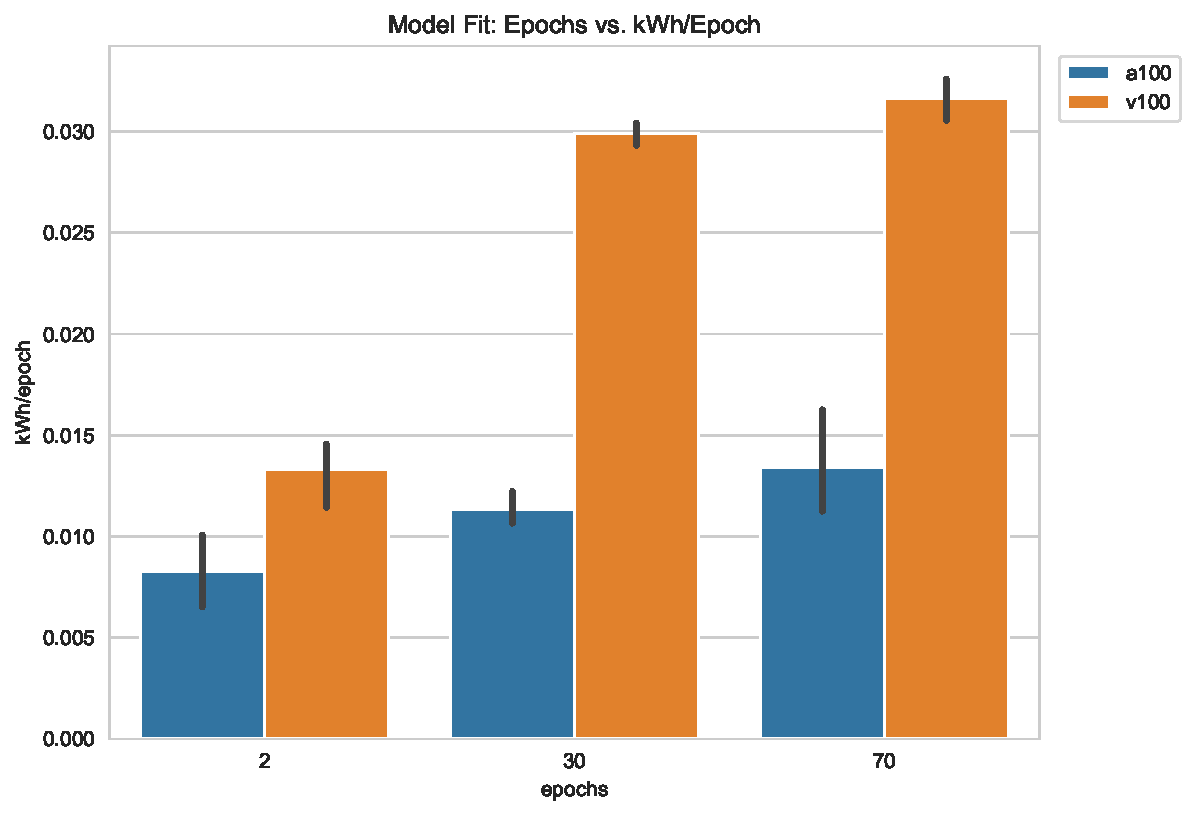
\includegraphics[width=1.0\linewidth]{images/model_fit_kWh_per_epoch.pdf}
     %   {\bf (D)} model fit kWh per epoch
     %\end{minipage}


\begin{comment}
\begin{figure}[p]

  \begin{center}
     \begin{minipage}[t]{0.30\textwidth}
        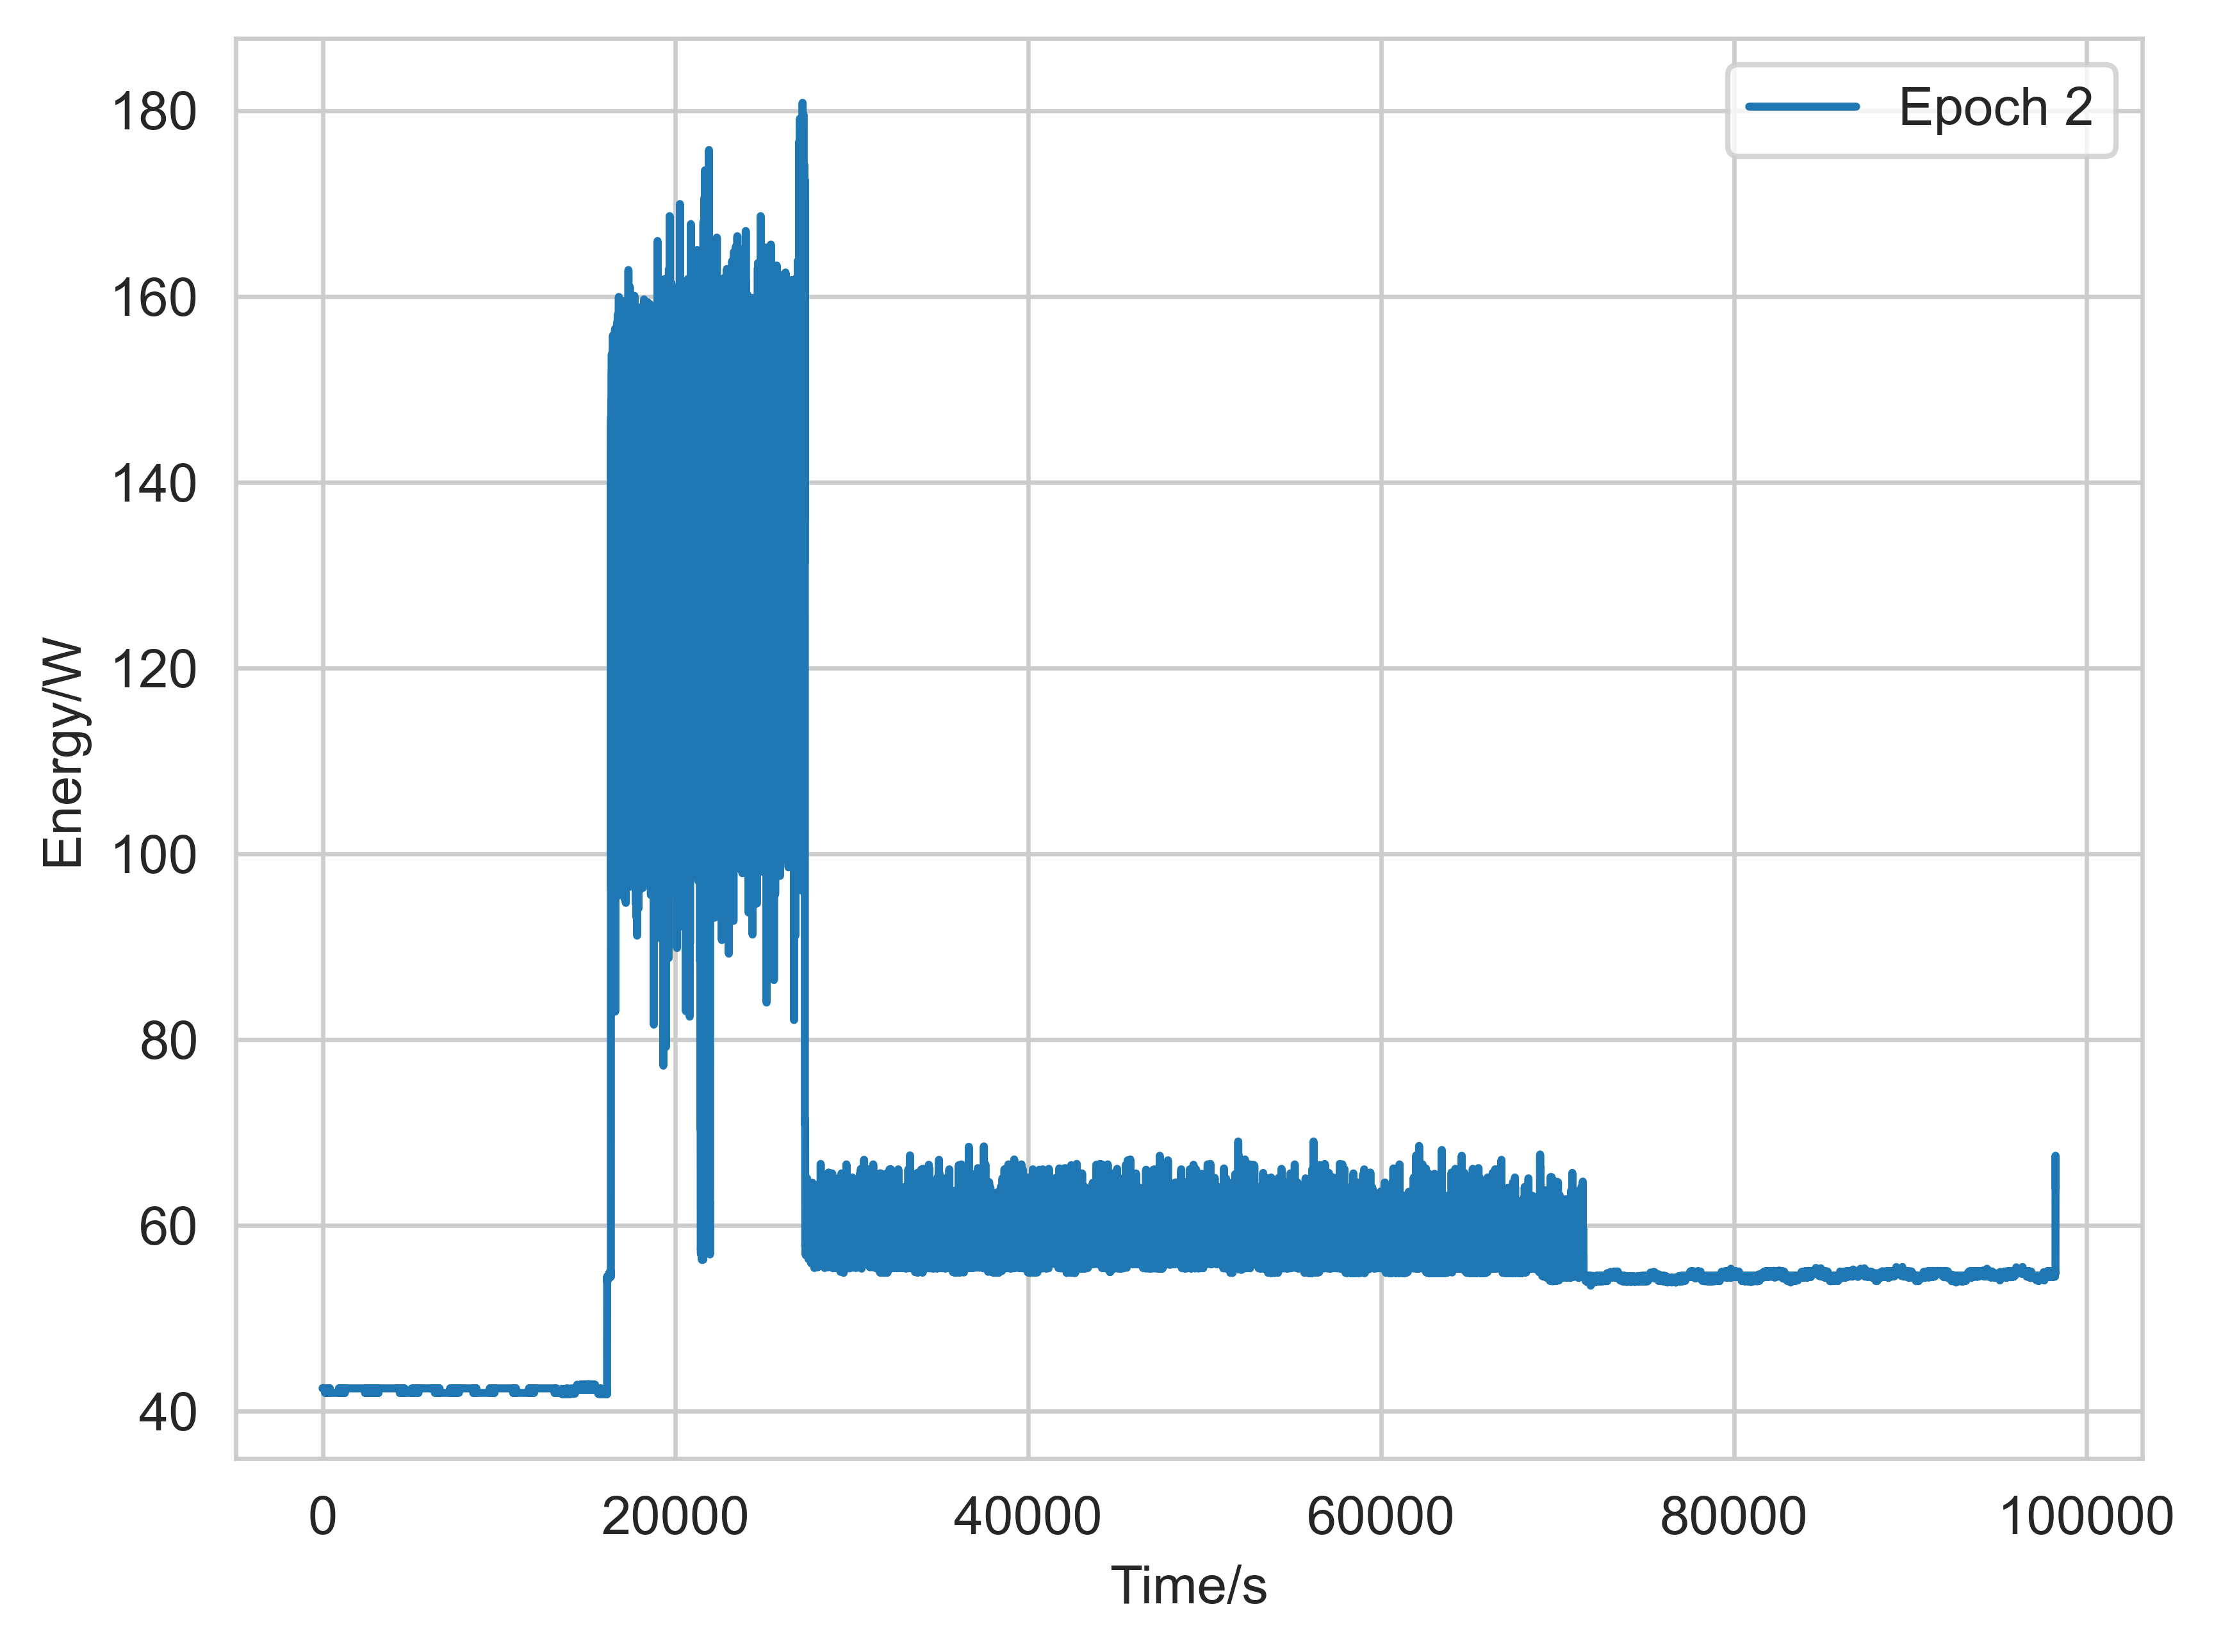
\includegraphics[width=1.0\linewidth]{images/card-name-v100-gpu-count-1-cpu-num-6-mem-32gb-repeat-1-tfttransformerepochs-2.png}
        {\bf (A)} Energy consumption for 2 epochs training and validation.
     \end{minipage}
     \ \
     \begin{minipage}[t]{0.30\textwidth}
        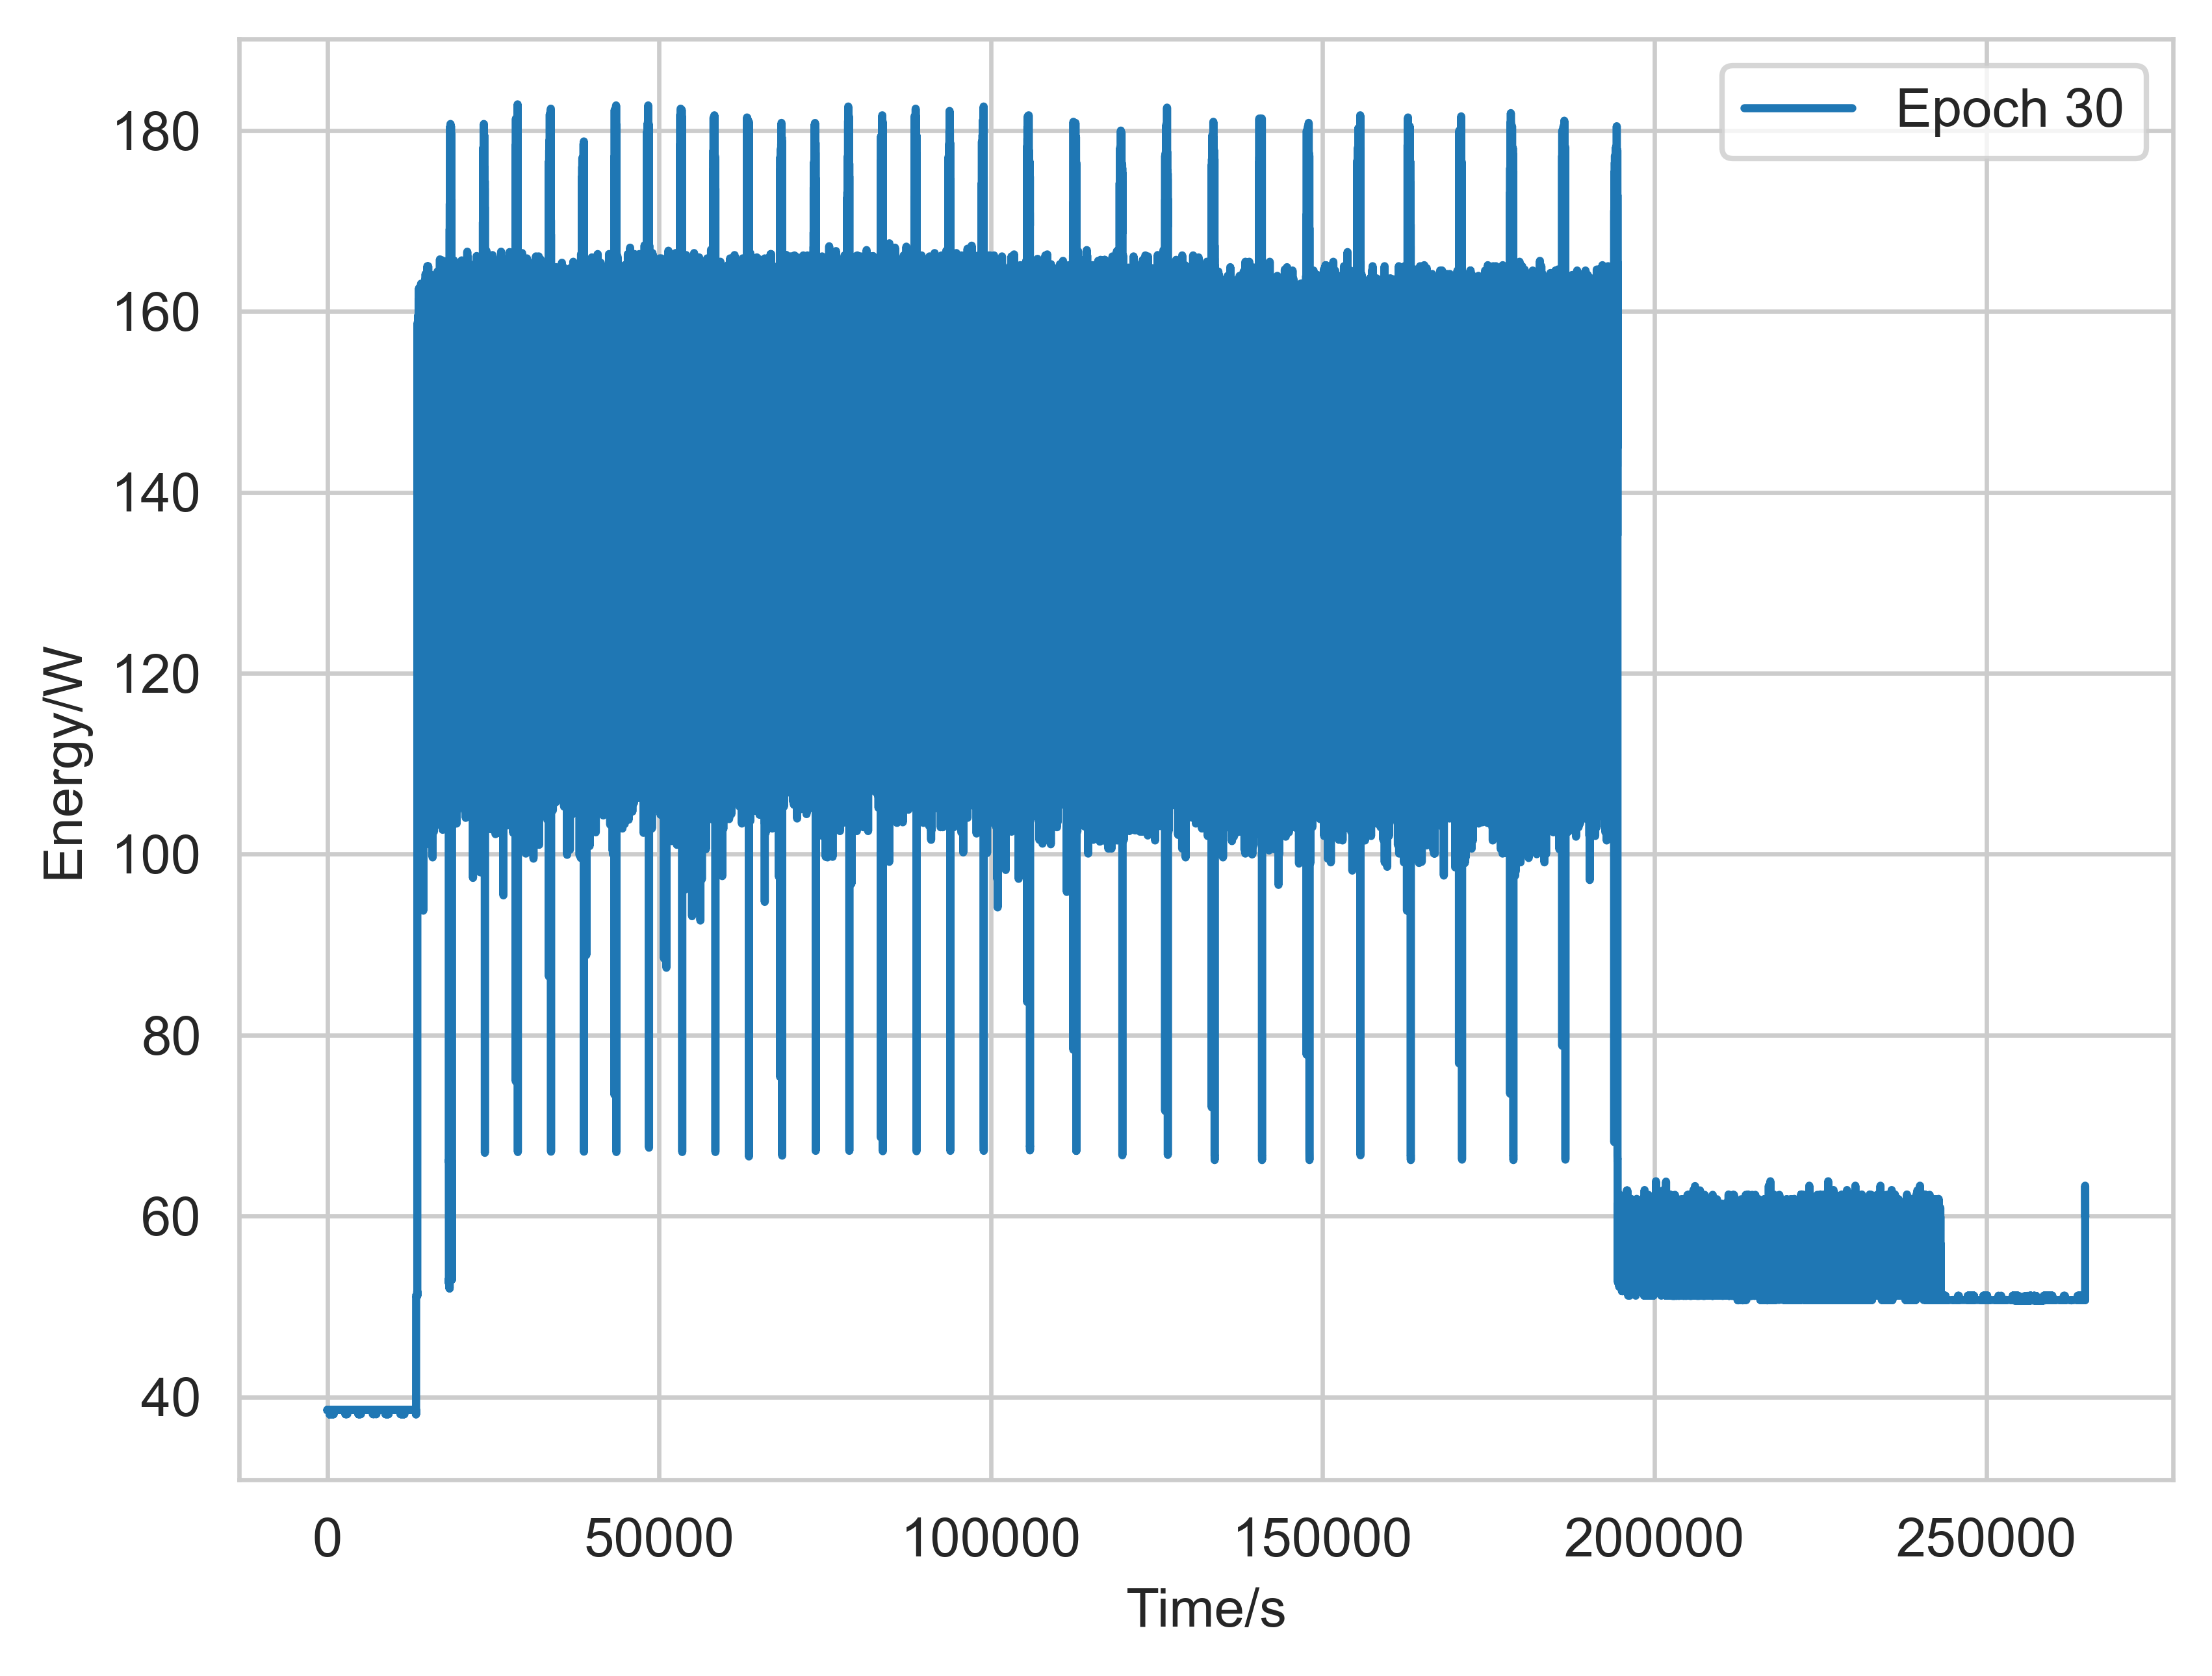
\includegraphics[width=1.0\linewidth]{images/card-name-v100-gpu-count-1-cpu-num-6-mem-32gb-repeat-1-tfttransformerepochs-30.png}
        {\bf (B)} Energy consumption for 30 epochs training and validation.
     \end{minipage}
     \ \
     \begin{minipage}[t]{0.30\textwidth}
        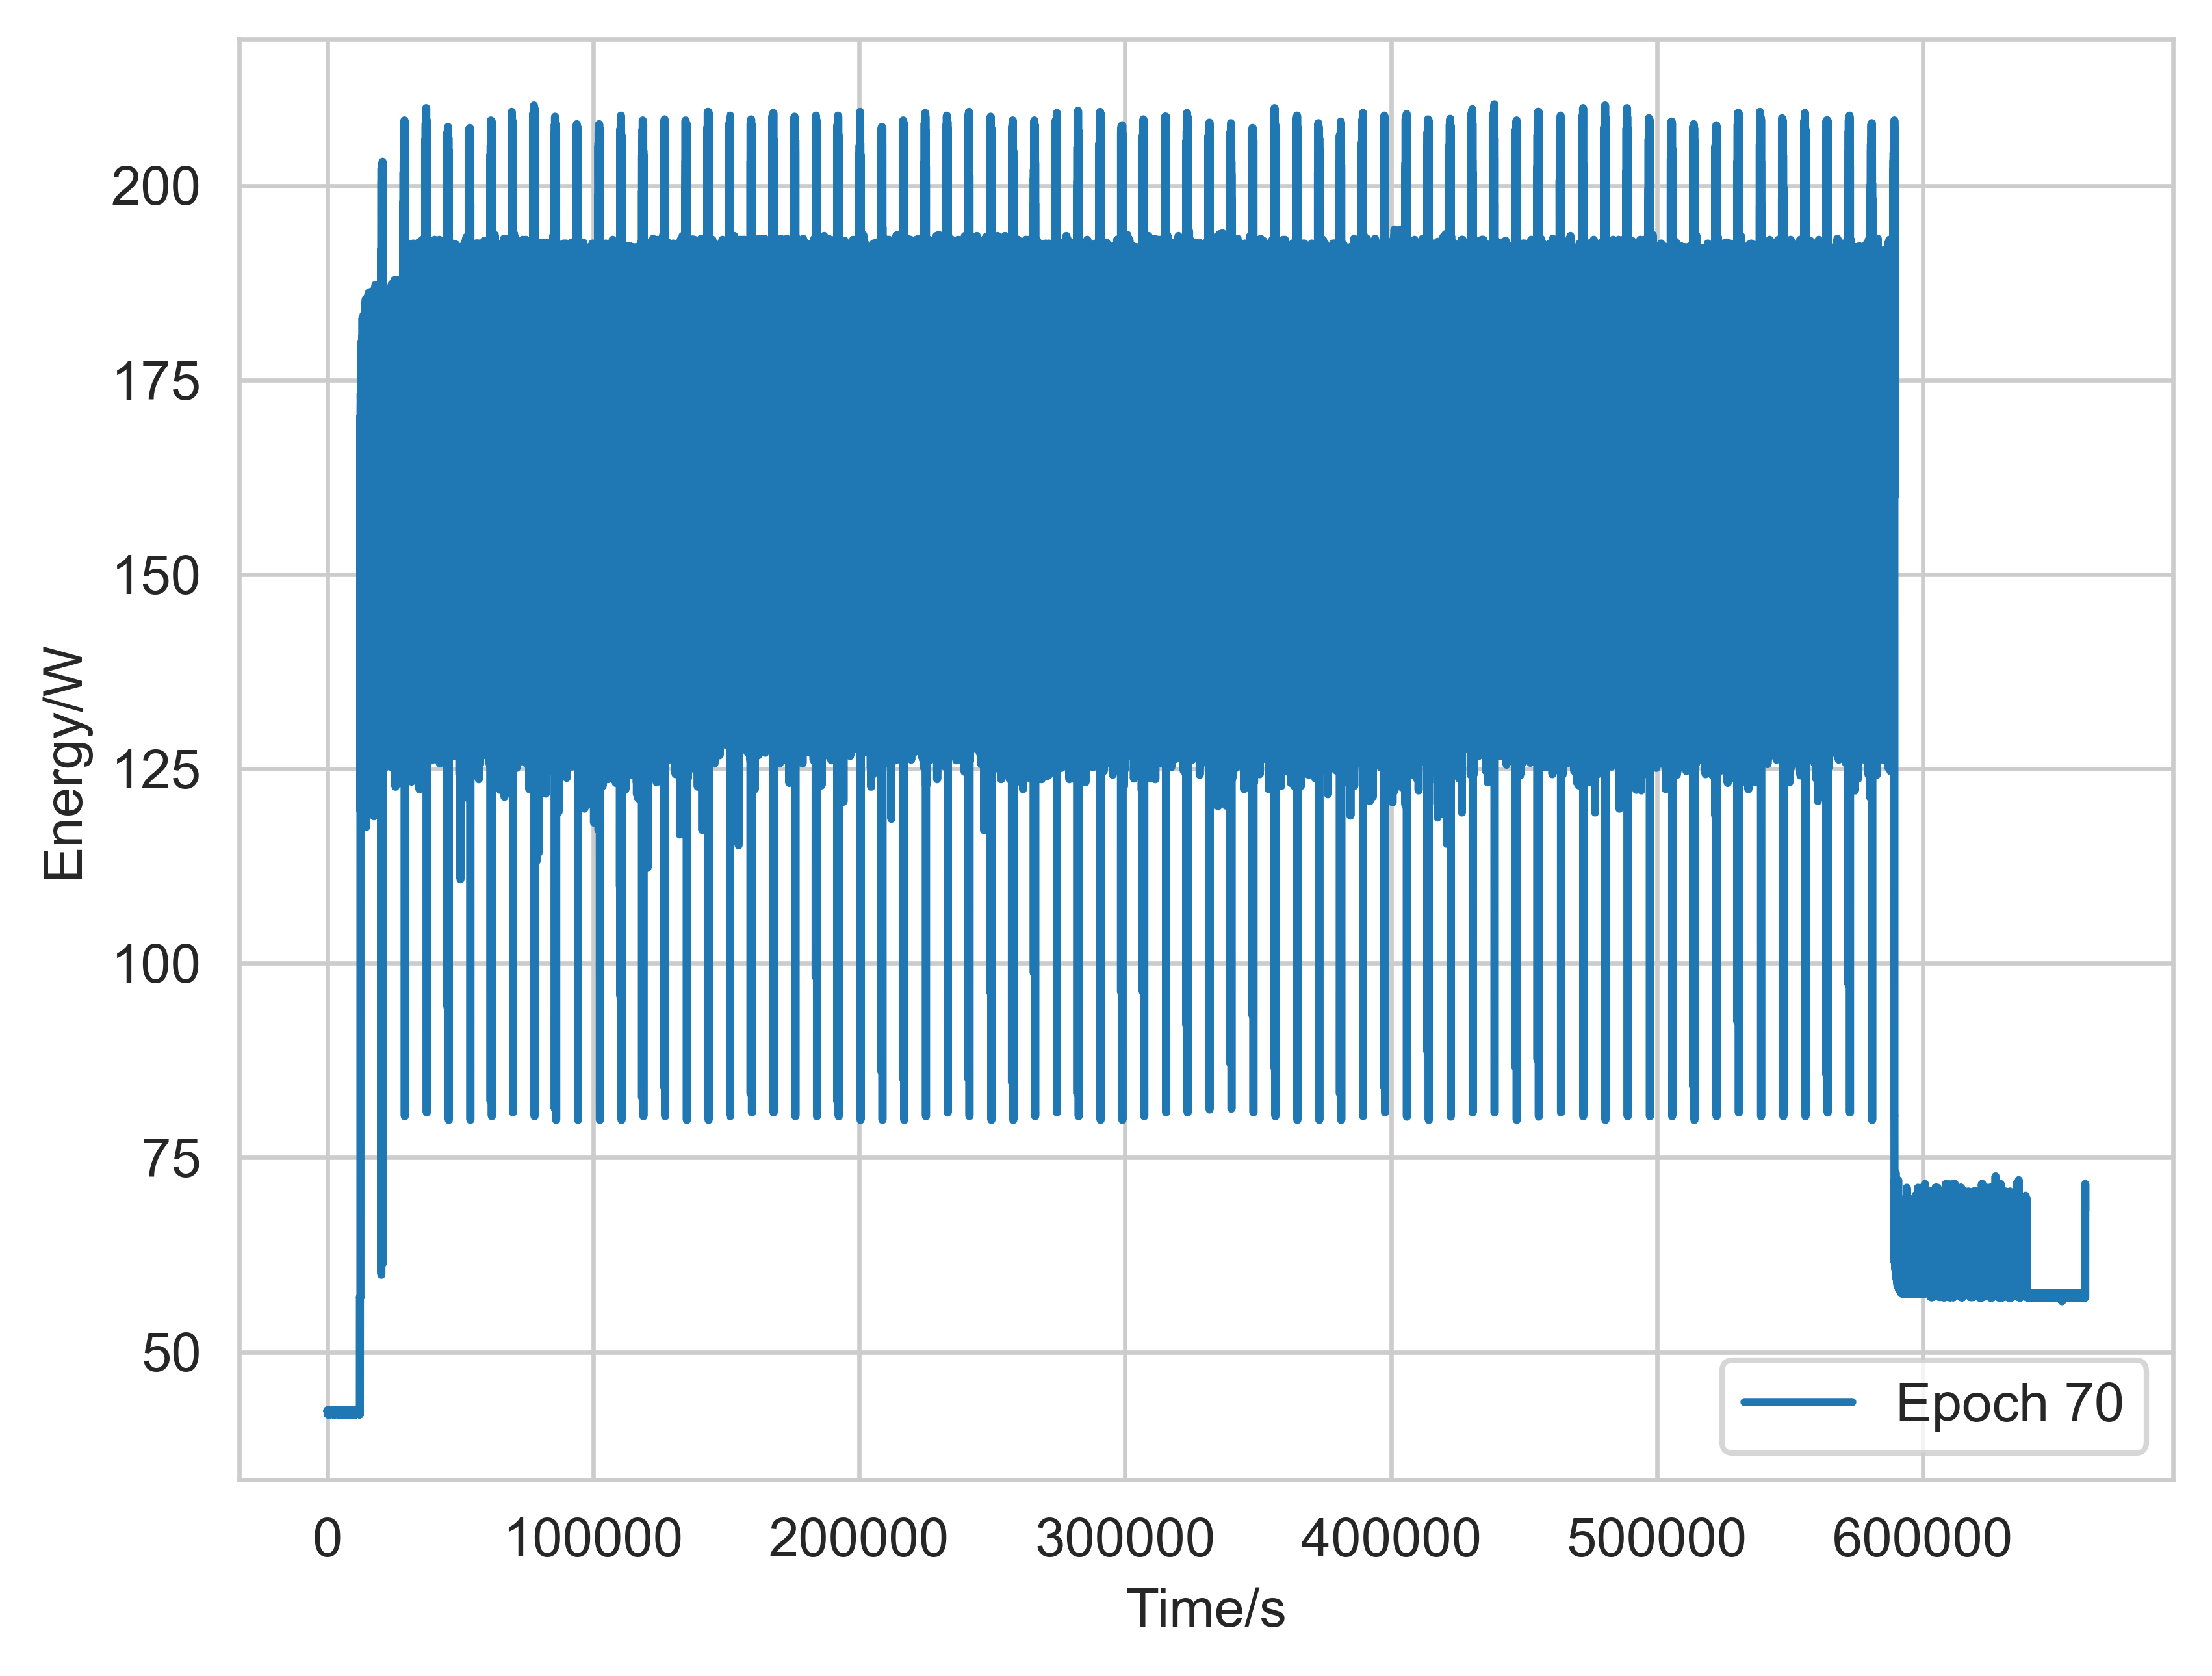
\includegraphics[width=1.0\linewidth]{images/card-name-v100-gpu-count-1-cpu-num-6-mem-32gb-repeat-1-tfttransformerepochs-70.png}
        {\bf (C)} Energy consumption for 70 epochs training and validation.
     \end{minipage}
  \end{center}

  \caption {Energy monitoring for 2, 30, and 70 epochs for training and validation for the A100.}
  \label{fig:energy}

\end{figure}
\end{comment}

\begin{figure}[p]

  \begin{center}
     \begin{minipage}[t]{0.30\textwidth}
        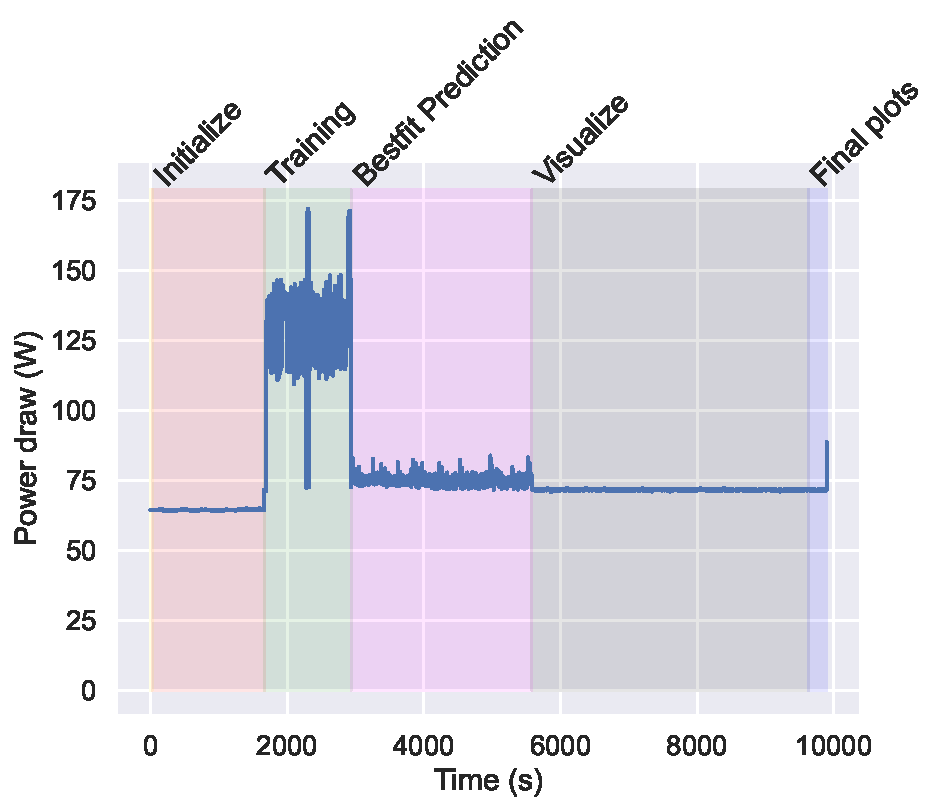
\includegraphics[width=1.0\linewidth]{images/a100-shaded-energy-2-epochs.pdf}
        {\bf (A)} Energy consumption for 2 epochs training and validation.
     \end{minipage}
     \ \
     \begin{minipage}[t]{0.30\textwidth}
        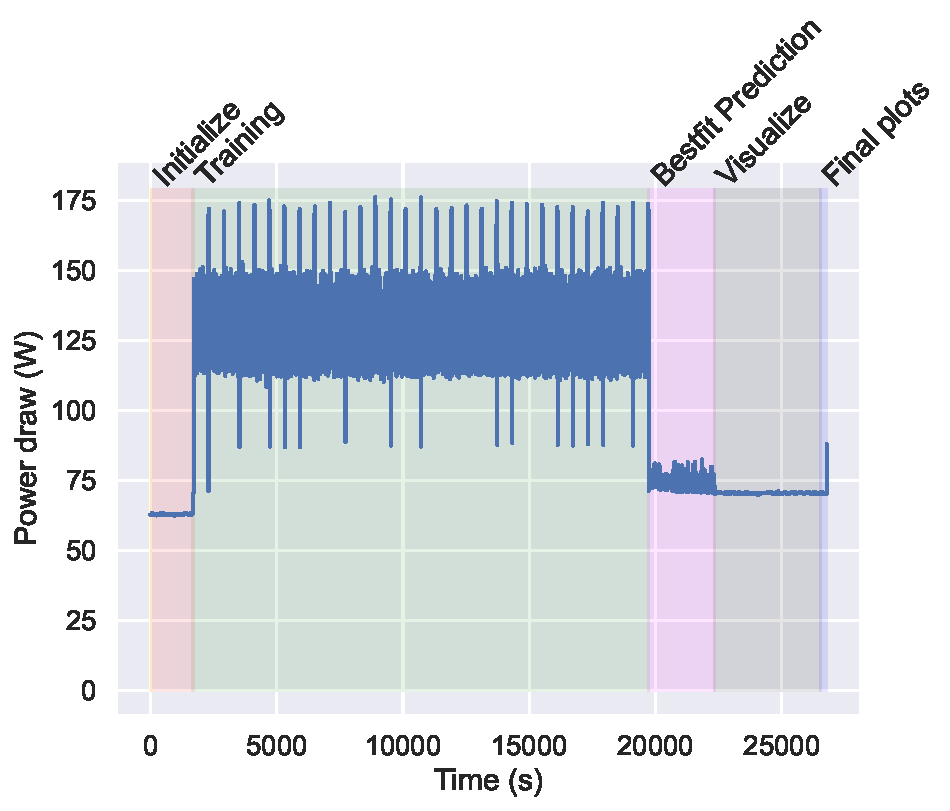
\includegraphics[width=1.0\linewidth]{images/a100-shaded-energy-30-epochs.pdf}
        {\bf (B)} Energy consumption for 30 epochs training and validation.
     \end{minipage}
     \ \
     \begin{minipage}[t]{0.30\textwidth}
        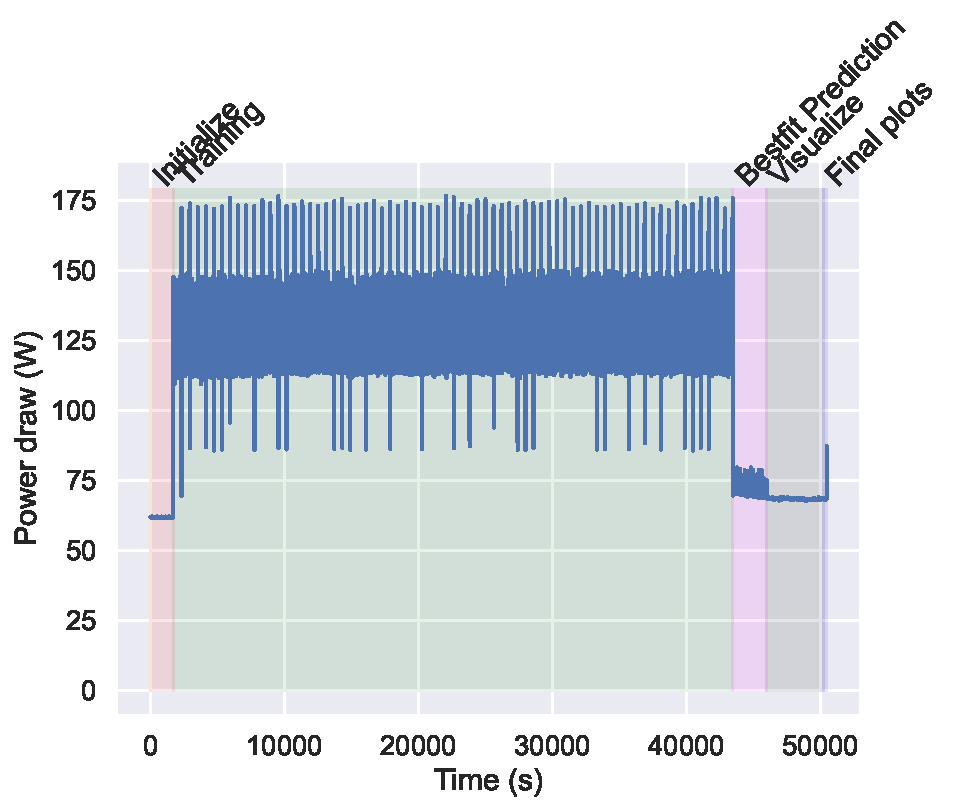
\includegraphics[width=1.0\linewidth]{images/a100-shaded-energy-70-epochs.pdf}
        {\bf (C)} Energy consumption for 70 epochs training and validation.
     \end{minipage}
  \end{center}

  \caption {Energy monitoring for 2, 30, and 70 epochs for training and validation for the A100.}
  \label{fig:energy}

\end{figure}

\begin{comment}

  %images/v100-shaded-energy-25-epochs.pdf
  %images/v100-shaded-energy-29-epochs.pdf
  %images/v100-shaded-energy-33-epochs.pdf
  %images/v100-shaded-energy-35-epochs.pdf



  \begin{figure}[p]

  \begin{center}
     \begin{minipage}[t]{0.30\textwidth}
        \includegraphics[width=1.0\linewidth]
        {\bf (A)} Energy trace for 2 epochs training and validation.
     \end{minipage}
     \ \
     \begin{minipage}[t]{0.30\textwidth}
        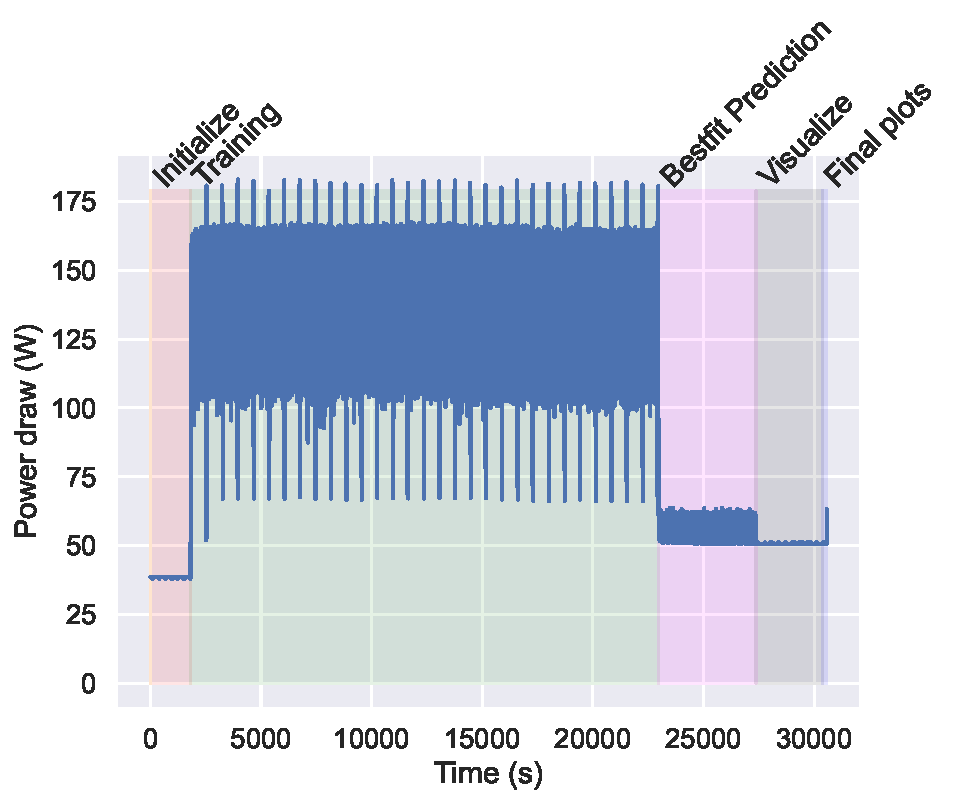
\includegraphics[width=1.0\linewidth]{images/v100-shaded-energy-30-epochs.pdf}
        {\bf (B)} Energy trace for 30 epochs training and validation.
     \end{minipage}
     \ \
     \begin{minipage}[t]{0.30\textwidth}
       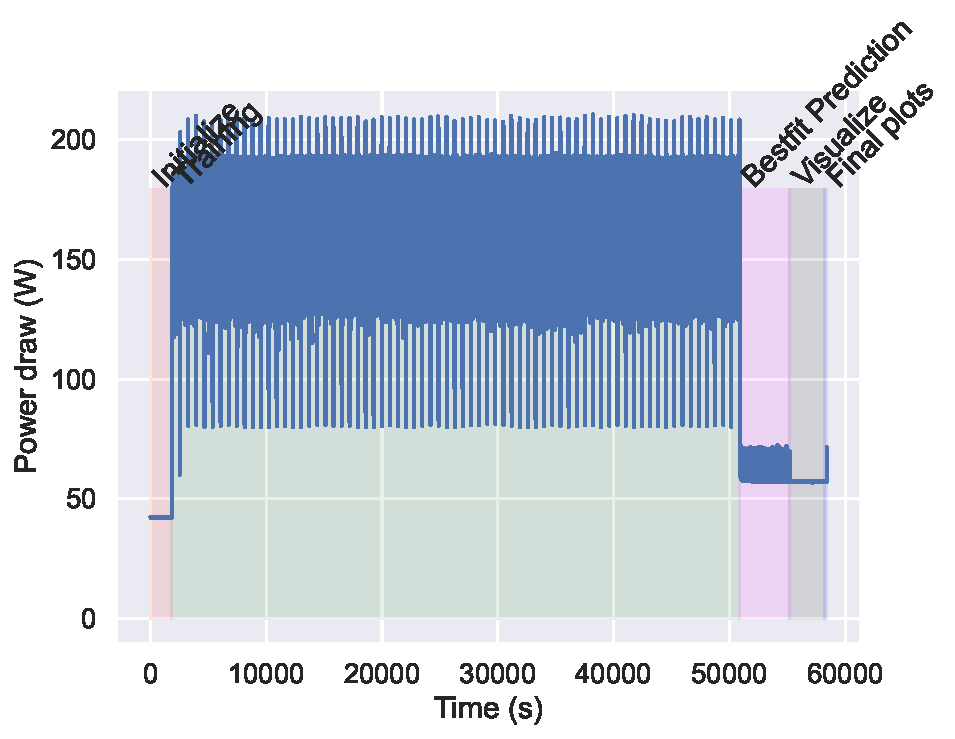
\includegraphics[width=1.0\linewidth]{images/v100-shaded-energy-70-epochs.pdf}
        {\bf (C)} Energy trace for 70 epochs training and validation.
     \end{minipage}
  \end{center}

  \caption {Energy monitoring for 2, 30, and 70 epochs for training and validation for the A100.}
  \label{fig:energy}

  \end{figure}
\end{comment}
